\documentclass[11pt]{article}
\usepackage[utf8]{inputenc}
\usepackage[english]{babel}
\usepackage{graphicx}
\usepackage[T1]{fontenc}
%\usepackage{amssymb,amsmath,graphicx}
\usepackage{amsfonts}
\usepackage{amsmath}
\usepackage{amssymb}
\usepackage{tabularx}
\usepackage{graphicx}
\usepackage{epsfig}
\usepackage{url}
%\usepackage[margin=1.5cm]{geometry}
\usepackage{listings}
\usepackage{comment}
\usepackage{booktabs}
\usepackage{eurosym}
\usepackage{multirow}
\usepackage{multicol}
\usepackage{pgfgantt}
\usepackage{float}
\restylefloat{table}
\usepackage{setspace}
\usepackage{enumitem}
\usepackage[parfill]{parskip}
\usepackage{pdfpages}
\usepackage{perpage} %the perpage package
\MakePerPage{footnote} %the perpage package command
\usepackage[font={small,it}]{caption}
\usepackage[colorlinks=true]{hyperref}
\definecolor{mygreen}{RGB}{28,172,0} % color values Red, Green, Blue
\definecolor{mylilas}{RGB}{170,55,241}
\usepackage[font={small,it}]{caption}
\usepackage[toc,page]{appendix}
% For inserting Matlab code into Sharelatex
\definecolor{dkgreen}{rgb}{0,0.6,0}
\definecolor{gray}{rgb}{0.5,0.5,0.5}
\definecolor{mauve}{rgb}{0.58,0,0.82}
\lstset{frame=tb,
  language=Matlab,
  aboveskip=3mm,
  belowskip=3mm,
  showstringspaces=false,
  columns=flexible,
  basicstyle={\small\ttfamily},
  numbers=none,
  numberstyle=\tiny\color{gray},
  keywordstyle=\color{blue},
  commentstyle=\color{dkgreen},
  stringstyle=\color{mauve},
  breaklines=true,
  breakatwhitespace=true,
  tabsize=3,
  basicstyle=\footnotesize
}

\usepackage[a4paper, hmargin={1.5cm, 1.5cm}, vmargin={1.5cm, 1.5cm}]{geometry}

\renewcommand{\listfigurename}{Figures}
 
\renewcommand{\listtablename}{Tables}

\begin{document}

\begin{titlepage}

\newcommand{\HRule}{\rule{\linewidth}{0.5mm}} % Defines a new command for the horizontal lines, change thickness here

\center % Center everything on the page
 
%----------------------------------------------------------------------------------------
%	HEADING SECTIONS
%----------------------------------------------------------------------------------------


\textsc{\LARGE Technical University of Denmark}\\[1.5cm] % Name of your university/college
\textsc{\Large 02443 Stochastic Simulation}\\[0.5cm] % Major heading such as course name
\textsc{\large Report of Exercises}\\[0.5cm] % Minor heading such as course title
%\textsc{\large Data set: Forest fires in Portugal}\\[0.5cm]

%----------------------------------------------------------------------------------------
%	TITLE SECTION
%----------------------------------------------------------------------------------------

%\HRule \\[0.4cm]
%{ \huge \bfseries Supervised learning: Classification and regression}\\[0.4cm] % Title of your document
%\HRule \\[1.3cm]
 
%----------------------------------------------------------------------------------------
%	AUTHOR SECTION
%----------------------------------------------------------------------------------------

\begin{minipage}{0.4\textwidth}

\begin{flushleft} \large
\emph{Name:}\\
Sanaz Behboodi\\% Your name
Jie Xu \\

\end{flushleft}
\end{minipage}
~
\begin{minipage}{0.4\textwidth}
\begin{flushright} \large
\emph{Student \# :} \\
\textsc{s180176}\\
\textsc{s181238}% Supervisor's Name
\end{flushright}
\end{minipage}\\[2cm]

% If you don't want a supervisor, uncomment the two lines below and remove the section above
%\Large \emph{Author:}\\
%John \textsc{Smith}\\[3cm] % Your name

%----------------------------------------------------------------------------------------
%	DATE SECTION
%----------------------------------------------------------------------------------------

{\large \today}\\[2cm] % Date, change the \today to a set date if you want to be precise

%----------------------------------------------------------------------------------------
%	LOGO SECTION
%----------------------------------------------------------------------------------------


\includegraphics[scale=0.07]{Figures/dtu_logo.png}\\ % Include a department/university logo - this will require the graphicx package
 
%----------------------------------------------------------------------------------------

\vfill % Fill the rest of the page with whitespace

\end{titlepage}


\thispagestyle{empty}
 

\clearpage
 
\pagenumbering{arabic}


\section{Exercise 1: Random number generation}
The aim of this exercise is generating pseudo random numbers by a computer algorithm such that the output is a sequence of reals
or integers, which suppose to be uniformly distributed on $[0,1]$ and statistically independent.
\subsection{Linear Congruential Generator (LCG)}
In the first step of this exercise, Linear Congruential Generator (LCG) is implemented for generating $10000$ random numbers by
\begin{equation}
    x_i=mod(ax_{i-1}+c, M),              U_i=\frac{x_i}{M}
\end{equation}
Where a is a multiplier, c is a shift and M is modulus, then these numbers is presented by a histogram for 10 classes.
\begin{center}
    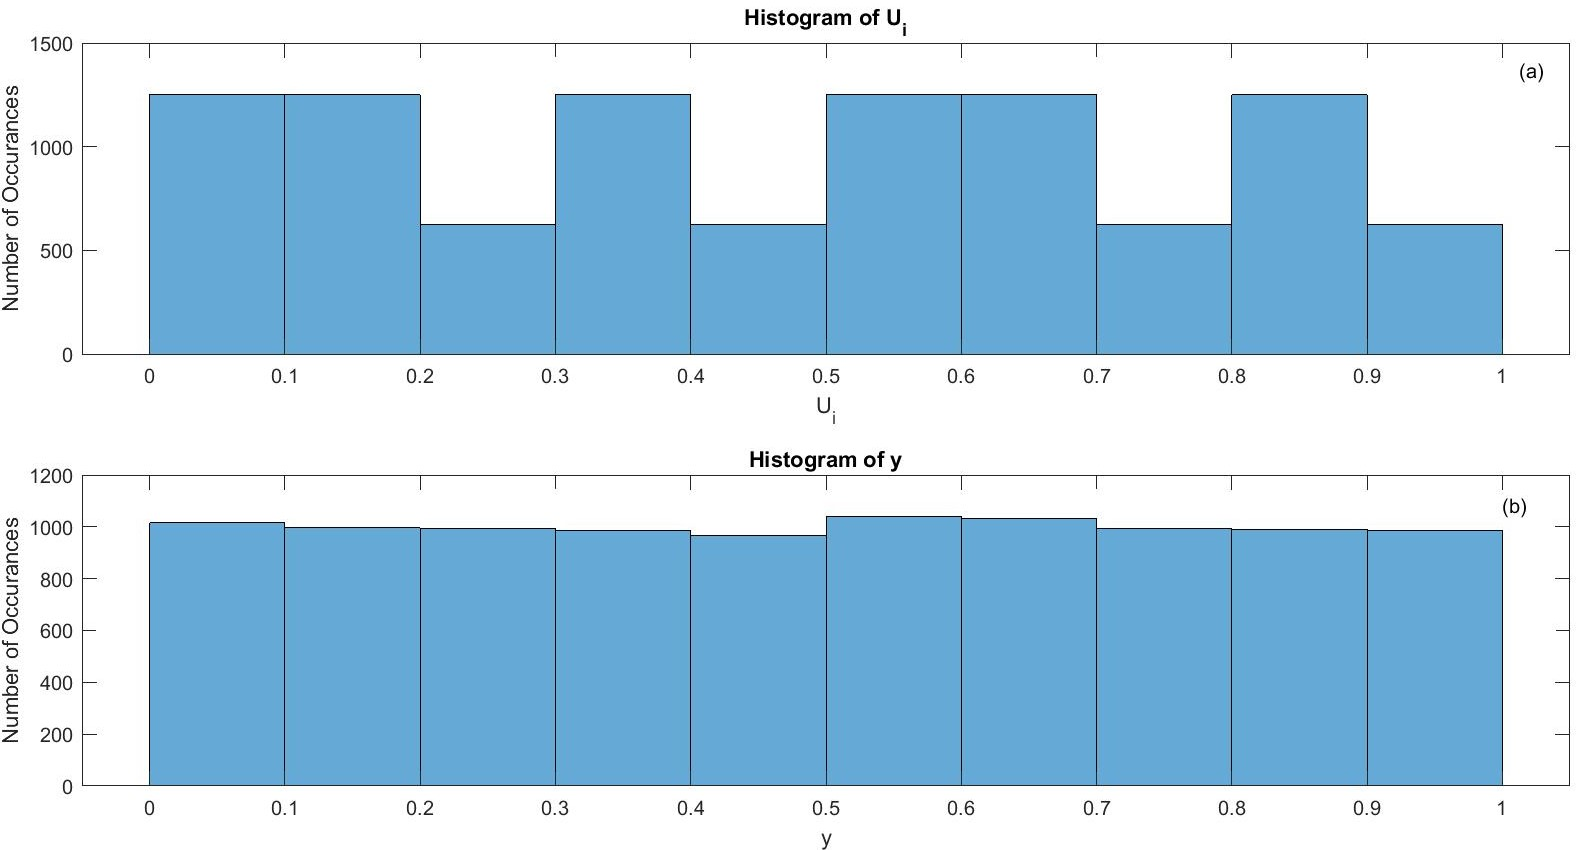
\includegraphics[scale=0.3]{Figures/figure1_1.jpg}\\
    \figuretitle{Figure 1: Histogram for U and Y.}
\end{center}\\
\\
Figure 1 show the histogram for U which generated by LCG and the histogram for Uniformly distributed random numbers.\\
\subsection{Evaluate the quality of the generators}
 The quality of the generators is evaluated  by graphical descriptive statistics (histogrammes, scatter plots) and statistical tests ($X^2$,Kolmogorov-Smirnov, run-tests, and correlation test).\\
 \begin{center}
    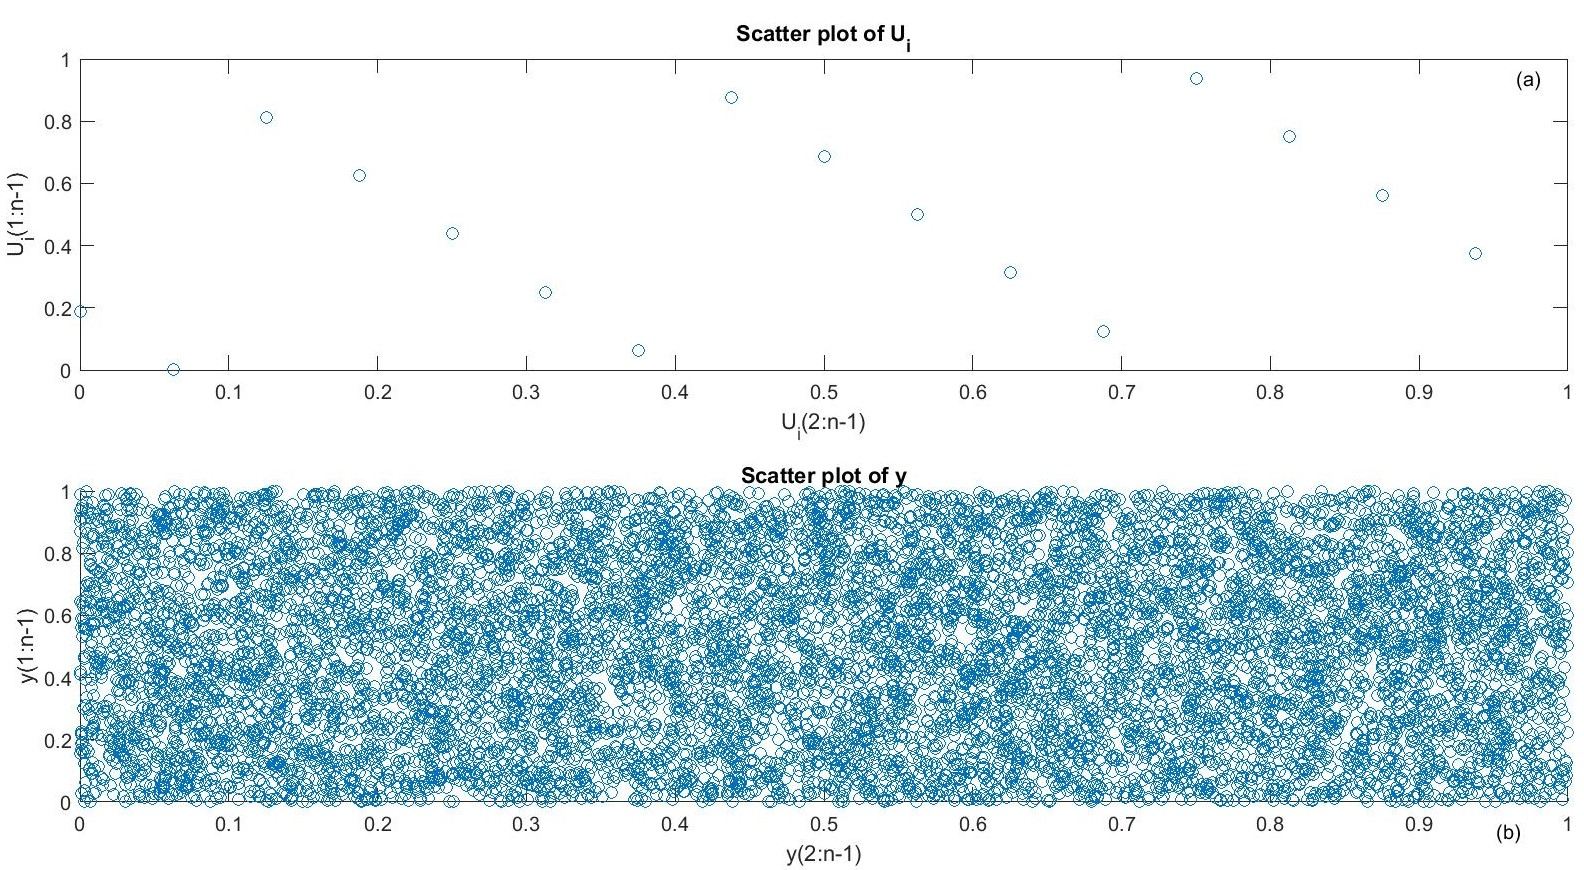
\includegraphics[scale=0.3]{Figures/figure1_2.jpg}\\
    \figuretitle{Figure 2: Scatter plot for U and Y.}
\end{center}\\
\\In this part of exercise, A chi-squared test ($\chi^2$ test) as a  statistical hypothesis test is implemented that is given by
\begin{equation}
  T=  \Sigma^{i=1}_{n_{classes}} =\frac{(n_{observed,i}-n_{expected,i})^2}{n_{expected,i}}
\end{equation}
The chi-squared test is used for the randomness of data to determine whether there is a significant difference between the expected frequencies and the observed frequencies in one or more categories.A chi-squared test can be used to attempt rejection of the null hypothesis that the data are independent.\\
%\lstinputlisting[language=matlab]{chi2test.m}
\\Now for testing the type of distribution of the random number generator, we implemented Kolmogorov-Smirnov test that can be used to compare a sample with a reference probability distribution. In this respect, the Kolmogorov–Smirnov statistic compares empirical distribution function $F_{n}(x)$  with hypothesized distribution $F(x)$ and it quantifies a distance that is given by
\begin{equation}
    D_n=sup_{x}{|F_{n}(x)-F(x)|}
\end{equation}
 \begin{center}
    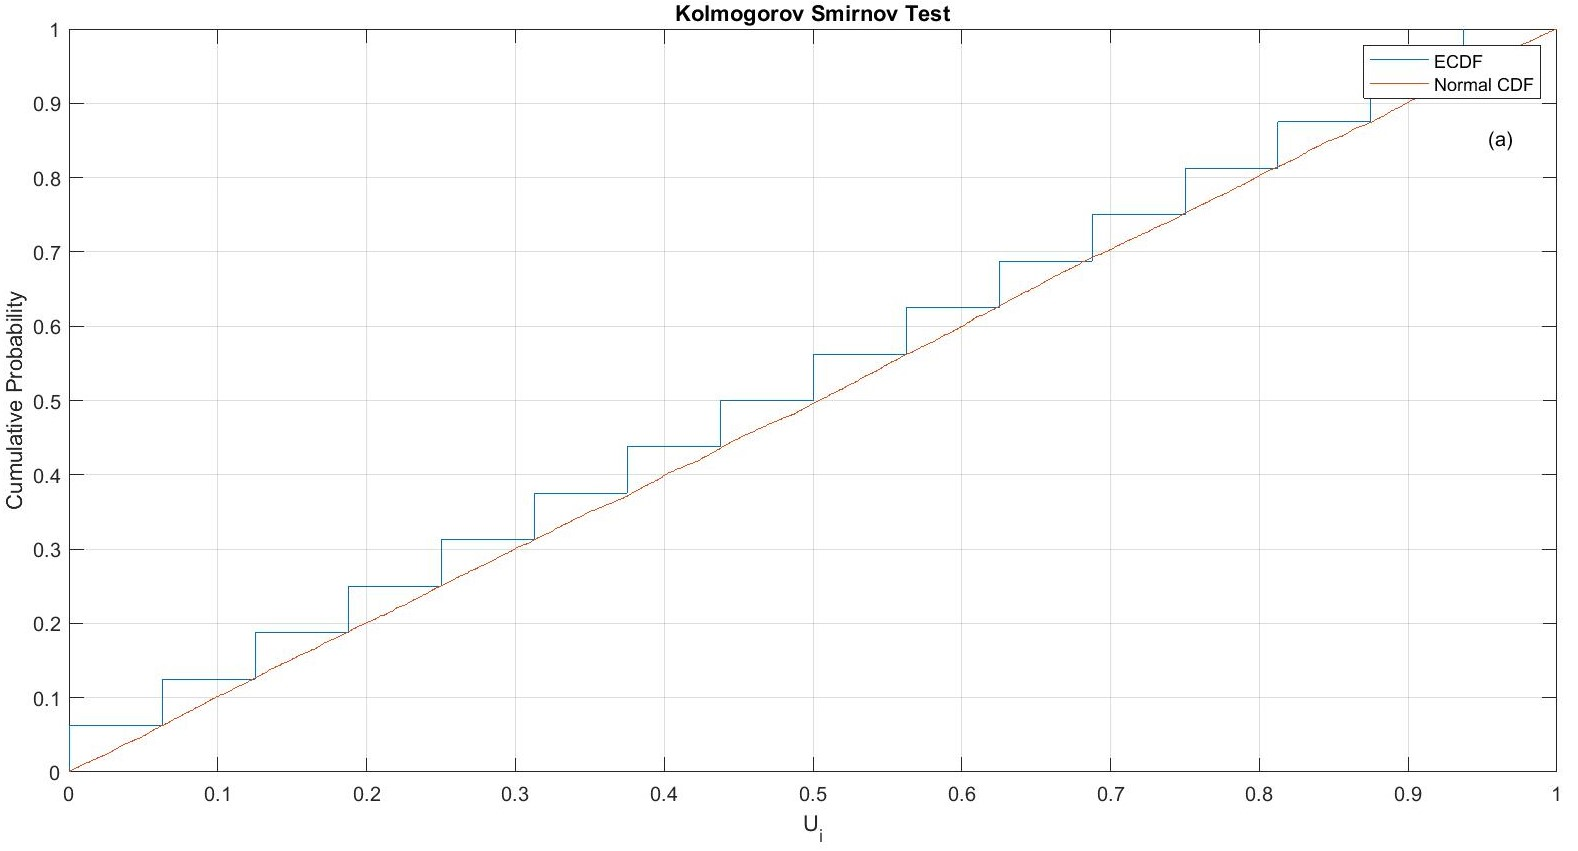
\includegraphics[scale=0.3]{Figures/figure1_3.jpg}\\
    \figuretitle{Figure 3: Kolmogorov–Smirnov Test .}
\end{center}\\
Figure 3 shows the Kolmogorov–Smirnov (KS) test.\\
Run test is other test which examines the arrangement of numbers in a sequence to test the hypothesis of independence and it can be used by comparing with the median.Let $n_1$ and $n_2$ be the number of individual observations above and below the mean, let b the total number of runs then the mean and variance of b can be expressed as 
\begin{equation}
    \mu_{b}=\frac{2n_{1}n_{2}}{2n_{1}+n_{2}}+1
\end{equation}
\begin{equation}
    \sigma^2_{b}=\frac{2n_{1}n_{2}(2n_{1}n_{2}-n_{1}-n_{2}}{(n_{1}+n_{2})^2(n_{1}+n_{2}-1)}
\end{equation}
$b$ is approximately normally distributed .\\
Correlation test is another independence test is given by
\begin{equation}
    C_{h}=\frac{1}{n-h}\Sigma^{i=1}_{n-h}U_{i}U_{i+h}\sim N(0.25,\frac{7}{144n})
\end{equation}






\section{Exercise 2: Generation of random variables-Discrete sample space}
The aim of this exercise is to generate the independent, discrete random variable $X_{i}$ having probability mass function 
\begin{equation}
    P\{X=x_{j}\} =p_{j},   j=0,1,...,\Sigma_{j}p_j=1
\end{equation}
To accomplish this, we assume, we have access to random number $U_{i}$ which is uniformly distributed over $(0,1)$ and finally transform $U_{i}$ to $X_{i}$. In this exercise we generated uniform random variables and we compared the results obtained in simulation with expected results with using histograms and tests.\\
\subsection{Geometric distribution}
first part of the exercise, Geometric distribution which is given by 
\begin{equation}
    F(n)=P(X\leq n)=1-(1-p)^n
\end{equation}
Where $X=\lfloor{(\frac{\log(U)}{\log(1-p)})}\lfloor+1$ with value of $p = 0.1$ is implemented and simulated for 10000 outcomes that shows in figure 4.\
\begin{center}
    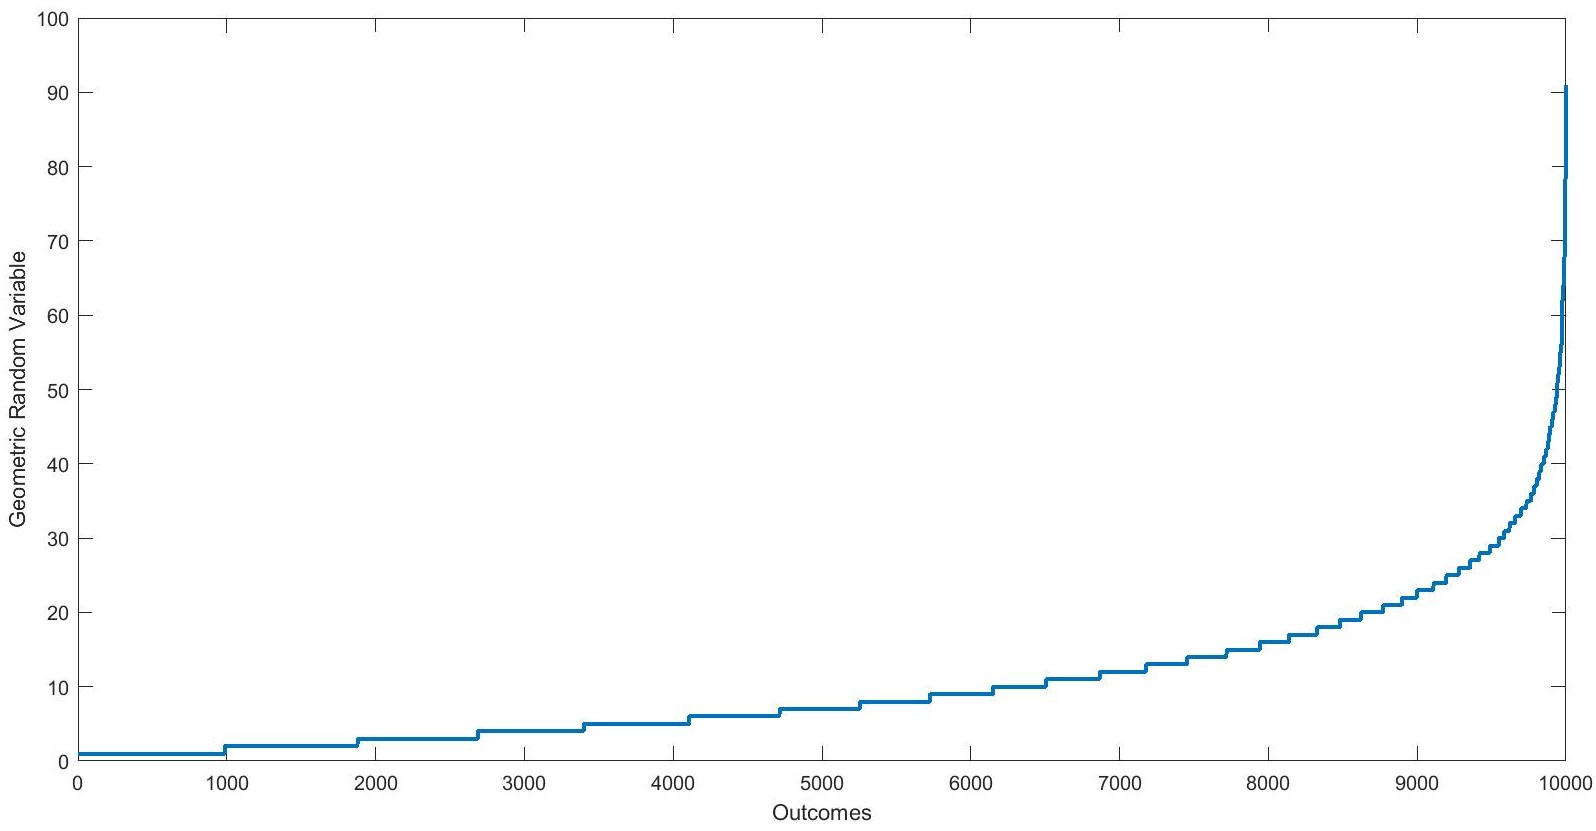
\includegraphics[scale=0.3]{Figures/figure2_1.jpg}\\
    \figuretitle{Figure 4:Geometric random variables for 10000 outcomes .}
\end{center}\\
\subsection{Simulate the 6 point distribution}

\begin{table}[h!]
\centering
\caption{6-point distribution.}
\label{summstats}
\begin{tabular}{|l|c|c|c|c|c|c|c|}
\hline
    X & 1 & 2 & 3 & 4 & 5 & 6  \\ \hline
    P_i & 7/48 & 5/48 & 1/8 & 1/16& 1/8 & 5/16 \\  \hline
\end{tabular}
\end{table}\\
\\
Figure 5 shows generating random variables and their histograms by By applying a direct(crude) method, rejection method and Alias method.\\
\begin{center}
    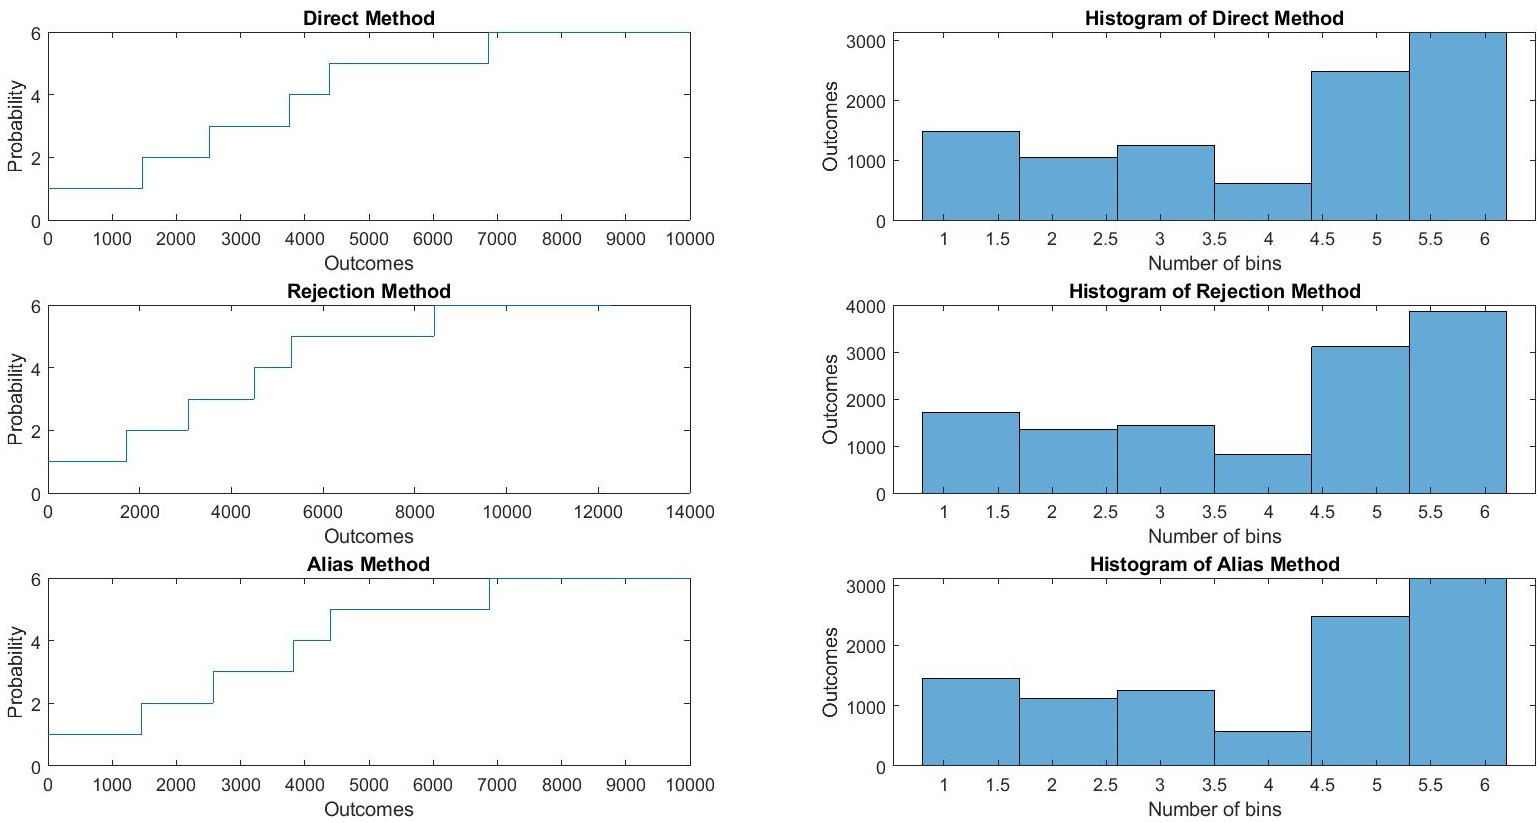
\includegraphics[scale=0.3]{Figures/figure2_2.jpg}\\
    \figuretitle{Figure 5: Different method for generating random variables and their histograms .}
\end{center}\\
\\Table2 presents result of  testing of generated uniform random variables with different methods .
\begin{table}[h!]
\centering
\caption{Testing of generated uniform random variables with different method .}
\label{summstats}
\begin{tabular}{|l|c|c|c|}
\hline
\textbf{Test}  & \multicolumn{1}{l|}{\textbf{Crude Method}} & \multicolumn{1}{l|}{\textbf{Rejection Method}}& \multicolumn{1}{l|}{\textbf{Alias Method}} \\ \hline

    $\chi^2$ Test & 1 & 1 & 1  \\ \hline
    KS Test & 1 & 1 & 1 \\  \hline
    Run Test & 0 & 1 & 1  \\ \hline
    CC Test & 1 & 1 & 1 \\  \hline
\end{tabular}
\end{table}\\
\\




\section{Exercise 3: Generation of random variables-Continuous sample space}
As same as last exercise the aim of this exercise is to generate the independent and continuous random variable by using the inverse transform approach and the rejection approach.

\subsection{Generated simulated value}
The first part of the exercise we generated simulated value from following distributions

1: Exponential distribution:

Let $X\sim \exp{\lambda}$ according inversion method, we have $X=F^{-1}(U)$\\
If $F(x)=1-\exp{(\lambda x)}$, then $F^{-1}(u)=-\frac{1}{\lambda}\log(1-u)$ (both 1-U and U are uniformly distributed.
\begin{equation}
    X=-\frac{\log(U)}{\lambda}\sim \exp{(\lambda)}
\end{equation}
\begin{center}
    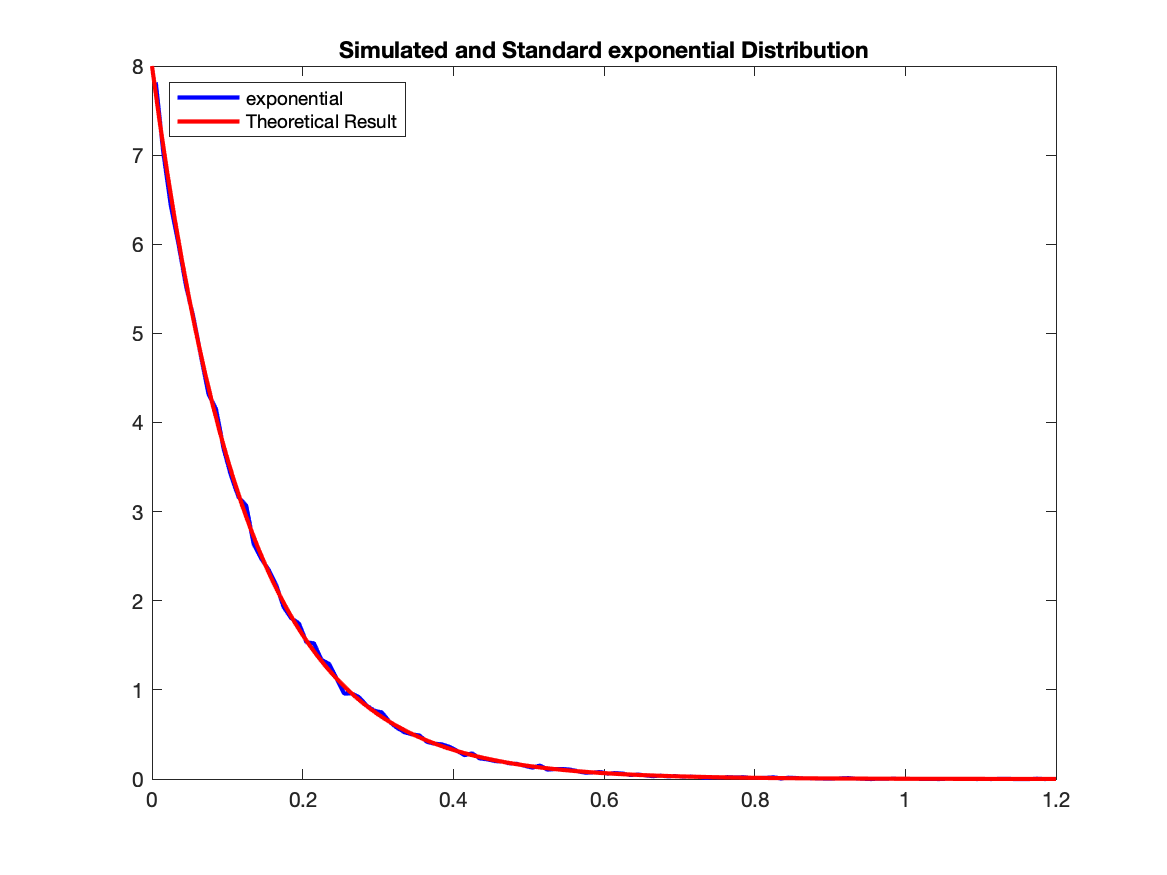
\includegraphics[scale=0.3]{Figures/figure3_1.png}\\
    \figuretitle{Figure 6: simulated values from Exponential distribution.}
\end{center}\\
\\
2: Normal distribution (at least with standard Box-Mueller):\\
Let $Z_{1},Z_{2}\sim N(0,1)$,the polar method or Box-Mueller is a way that transform from polar coordinate $\theta=2\piU_{2},r=\sqrt{-2\log(U_1)}$ into Cartesian coordinates$X=Z_{1}$ and $Y=Z_{2}$ which is given by
\begin{equation}
    Z_{1}=r\cos \theta   
\end{equation}
\begin{equation}
    Z_{2}= r\sin \theta
\end{equation}
\begin{center}
    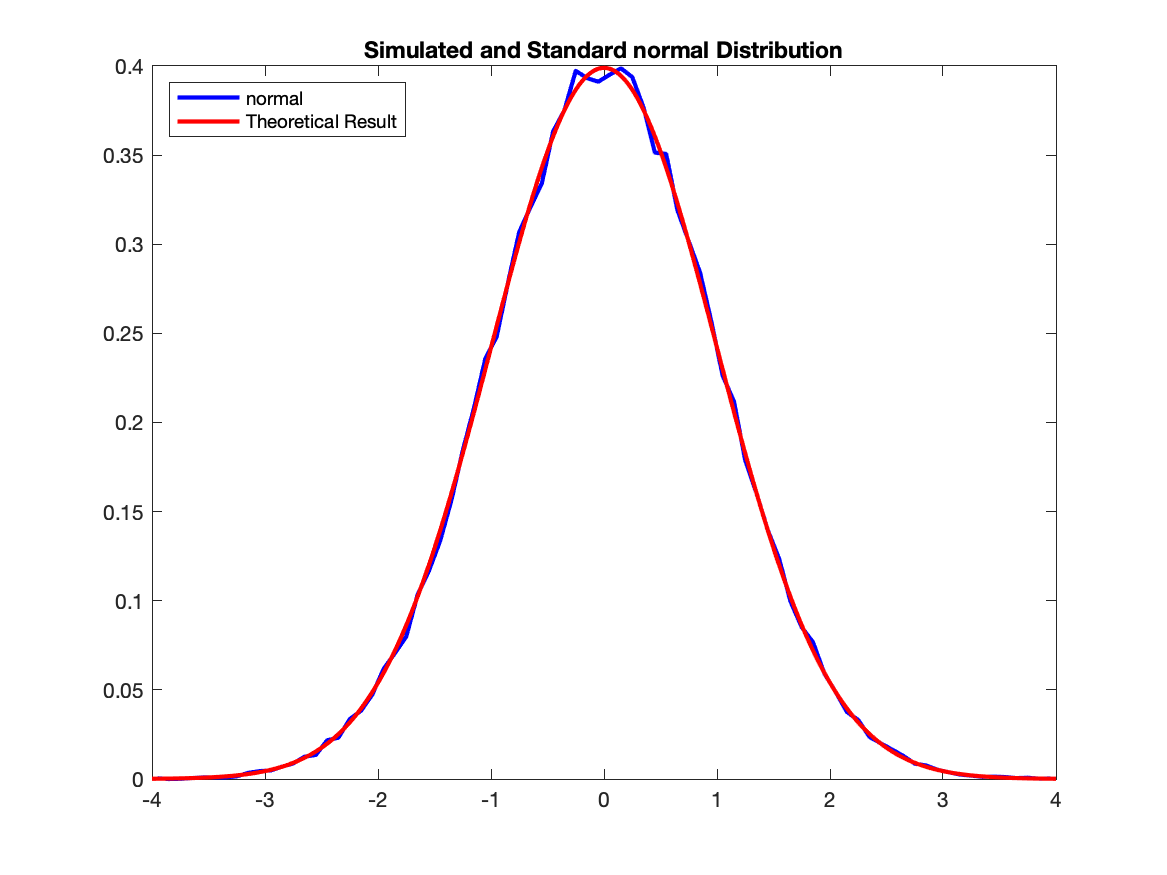
\includegraphics[scale=0.4]{Figures/figure3_2.png}\\
    \figuretitle{Figure 7: simulated values from Normal distribution.}
\end{center}\\
\\
3:Pareto distribution, with $\beta=1$ and different values of $K=2.05,2.5,3,4$\\
\begin{center}
    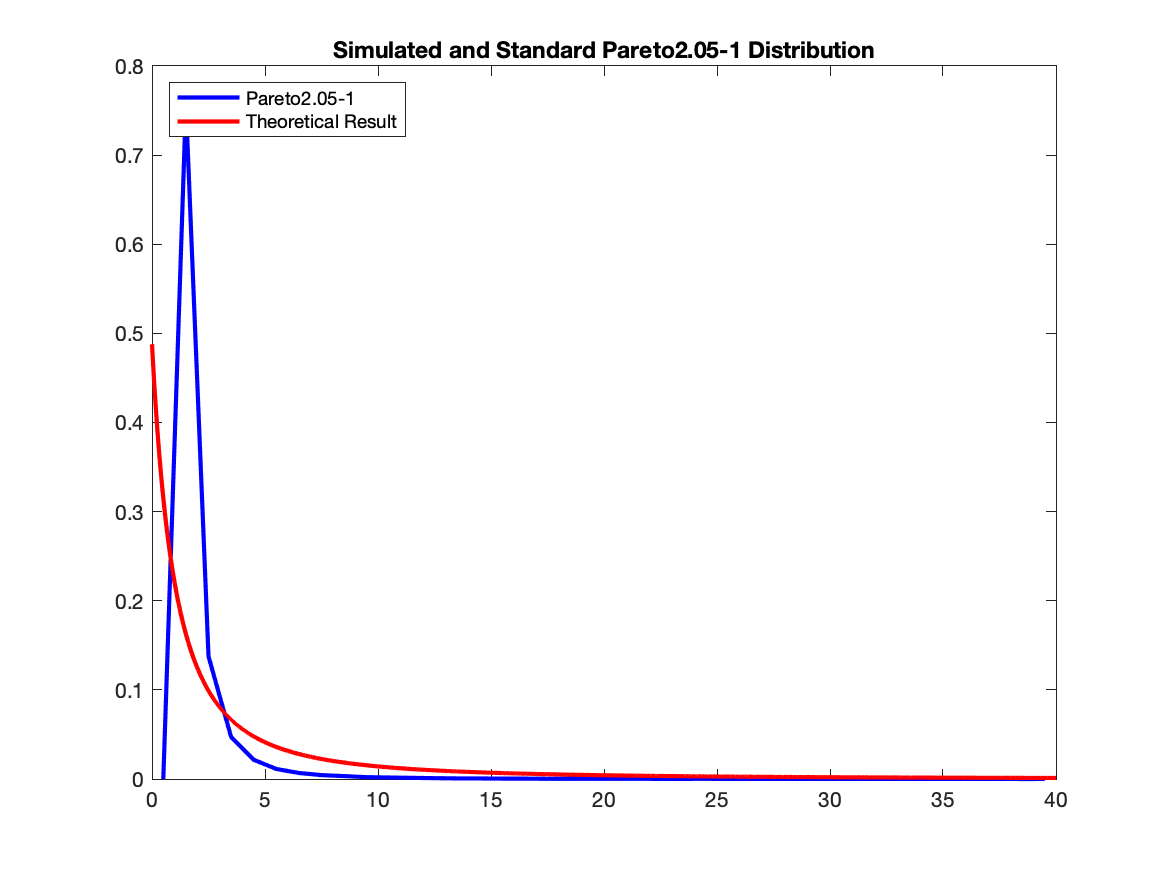
\includegraphics[scale=0.4]{Figures/figure3_3.png}\\
    \figuretitle{Figure 8: simulated values from Pareto distribution for K=2.05-1.}
\end{center}\\
\\
\begin{center}
    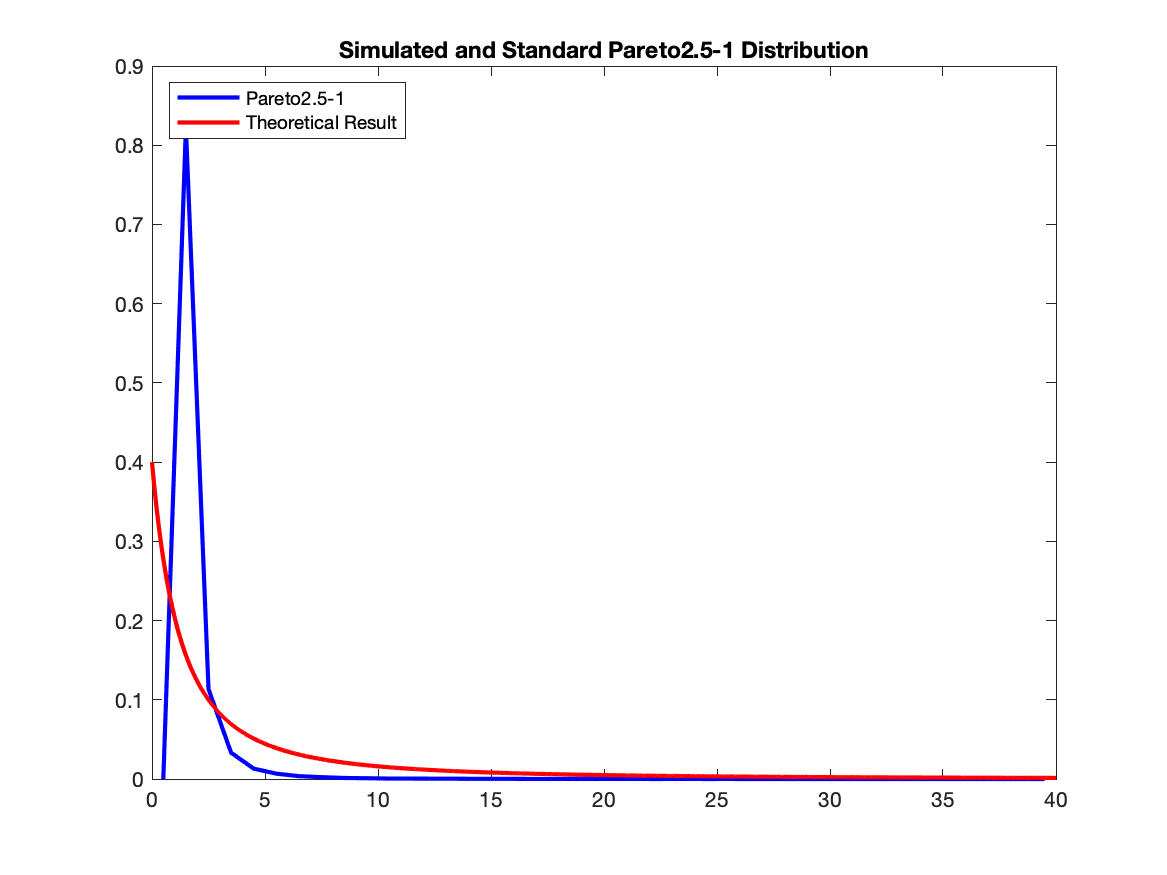
\includegraphics[scale=0.4]{Figures/figure3_4.png}\\
    \figuretitle{Figure 9: simulated values from Pareto distribution for K=2.5-1.}
\end{center}\\
\\
\begin{center}
    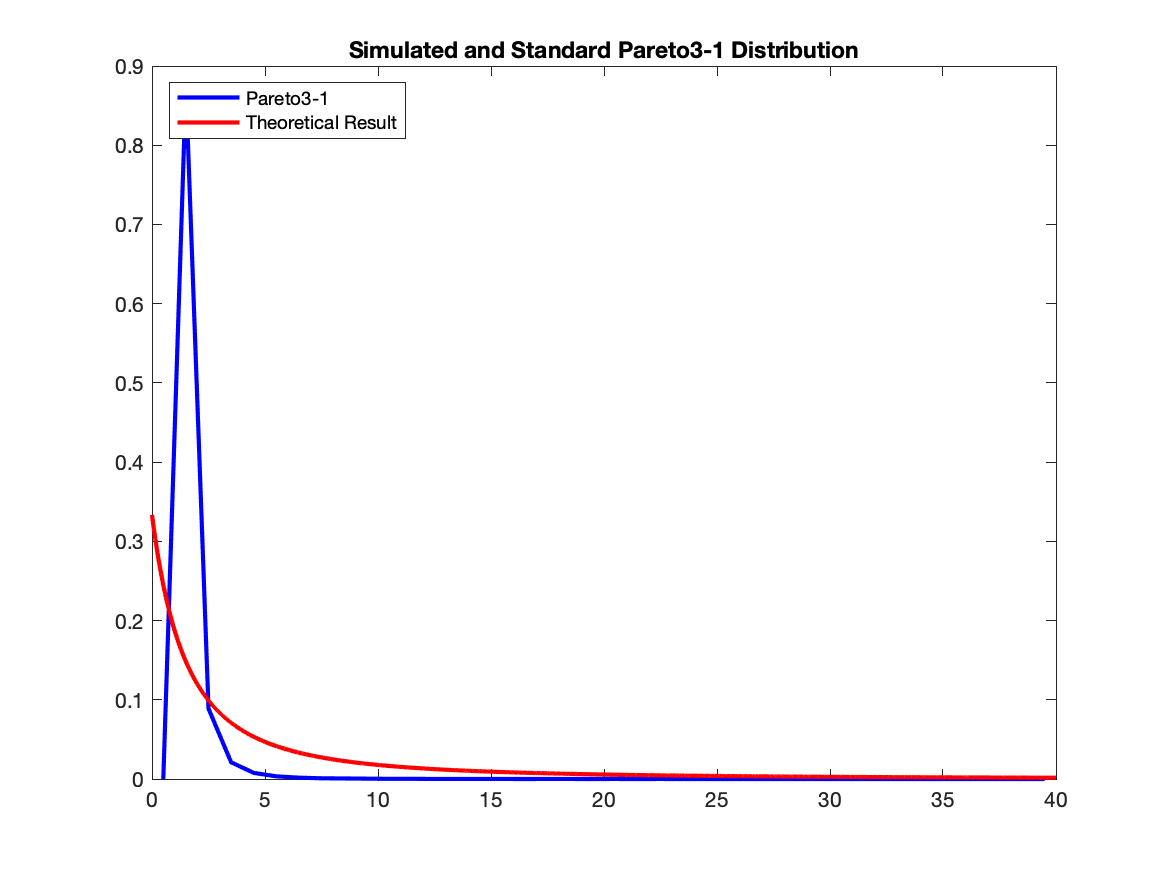
\includegraphics[scale=0.4]{Figures/figure3_5.png}\\
    \figuretitle{Figure 10: simulated values from Pareto distribution for K=3-1.}
\end{center}\\
\\
\begin{center}
    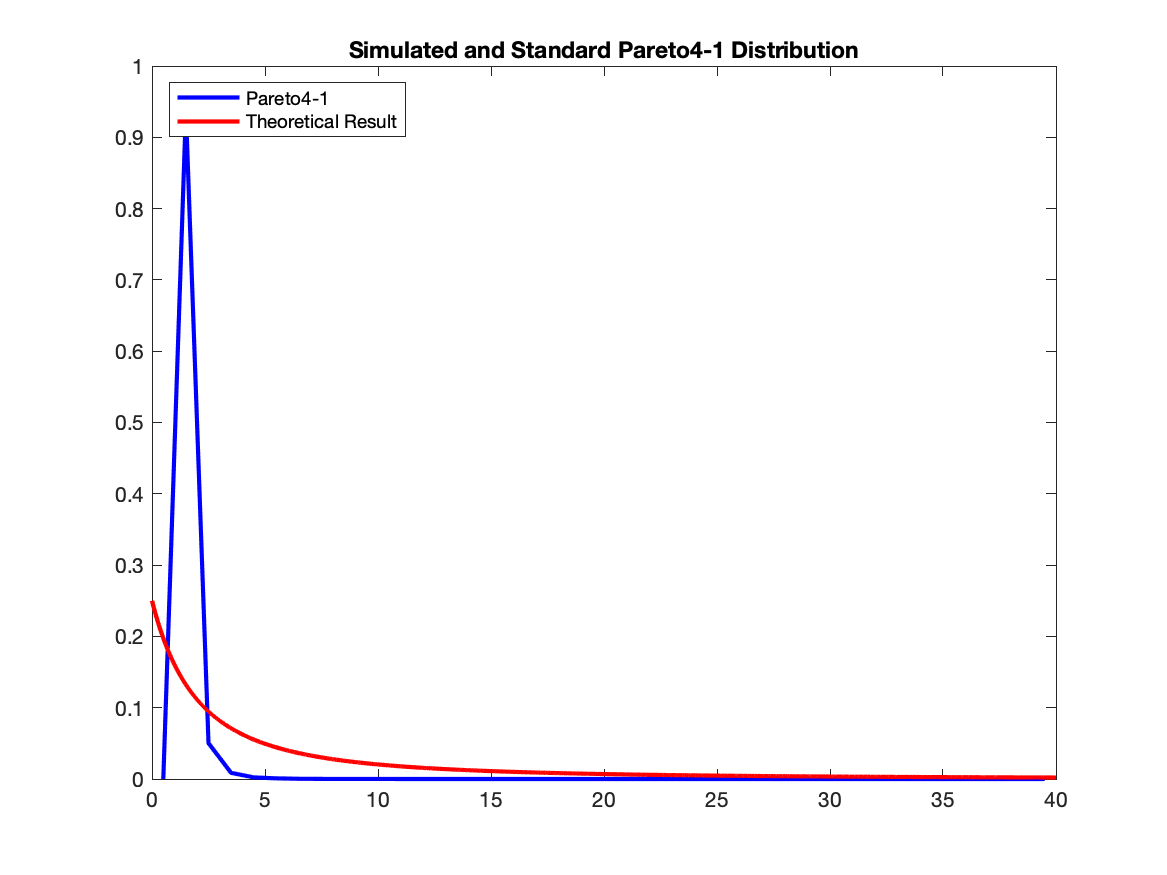
\includegraphics[scale=0.4]{Figures/figure3_6.png}\\
    \figuretitle{Figure 11: simulated values from Pareto distribution for K= 4-1.}
\end{center}\\
\\
\begin{center}
    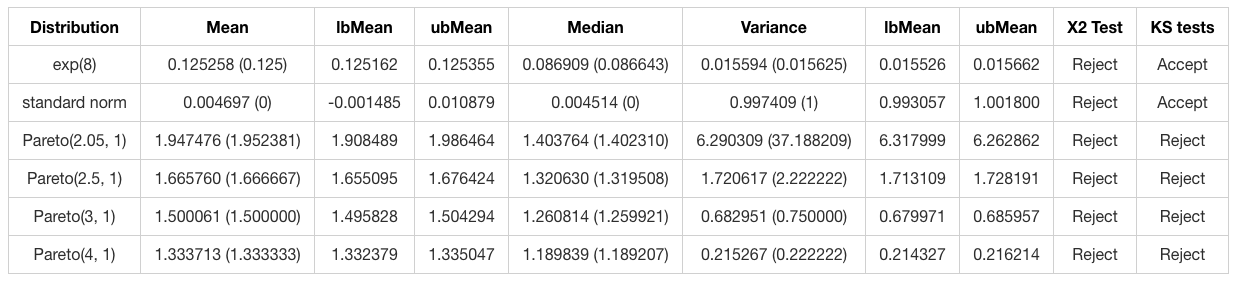
\includegraphics[scale=0.4]{Figures/figure3_7.png}\\
    \figuretitle{Table 3: Analysis and Test of the Simulation Result.}
\end{center}\\
\\








\section{Exercise 4: Discrete simulation/event-by-event}
In this exercise we write discrete event simulation program for a blocking system,with n service units and no waiting room.\\
First, the arrival process is modelled as a Poisson process and the service time distribution is modeled as exponential for $n = 10$(number of service units), mean service time = 8 time units, mean time between customers = 1 time unit and 10.000 customers, then record the fraction of blocked customers, and a confidence
interval for this fraction.\\
In the second part of this exercise, we substitute the arrival process with a renewal process with\\
1:Erlang distributed inter arrival times mean of 1\\
2:hyper exponential inter arrival times with $p_1 = 0.8$, $\lambda_1 = 0.8333$, $p_2 = 0.2$, $\lambda_2 = 5.0$.\\
Finally experiment with different service time distributions.
Suggestions are constant service time and Pareto distributed service times with k = 1.05 and k = 2.05.\\
All this results is presented in Table 4.\\

\begin{center}
    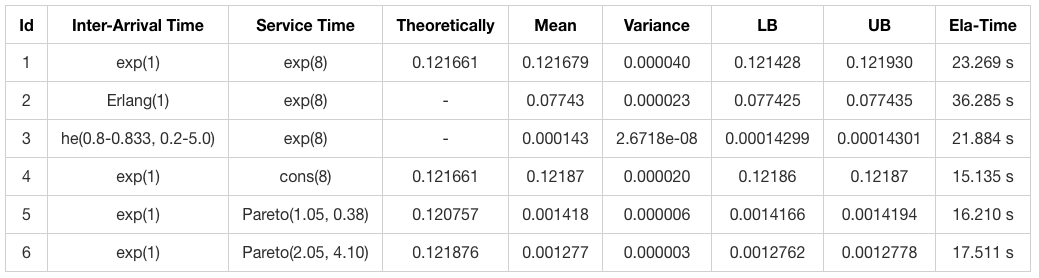
\includegraphics[scale=0.5]{Figures/figure4_1.png}\\
    \figuretitle{Table 4 :Discrete Event Simulation of Blocking System .}
\end{center}\\
\\
\begin{center}
    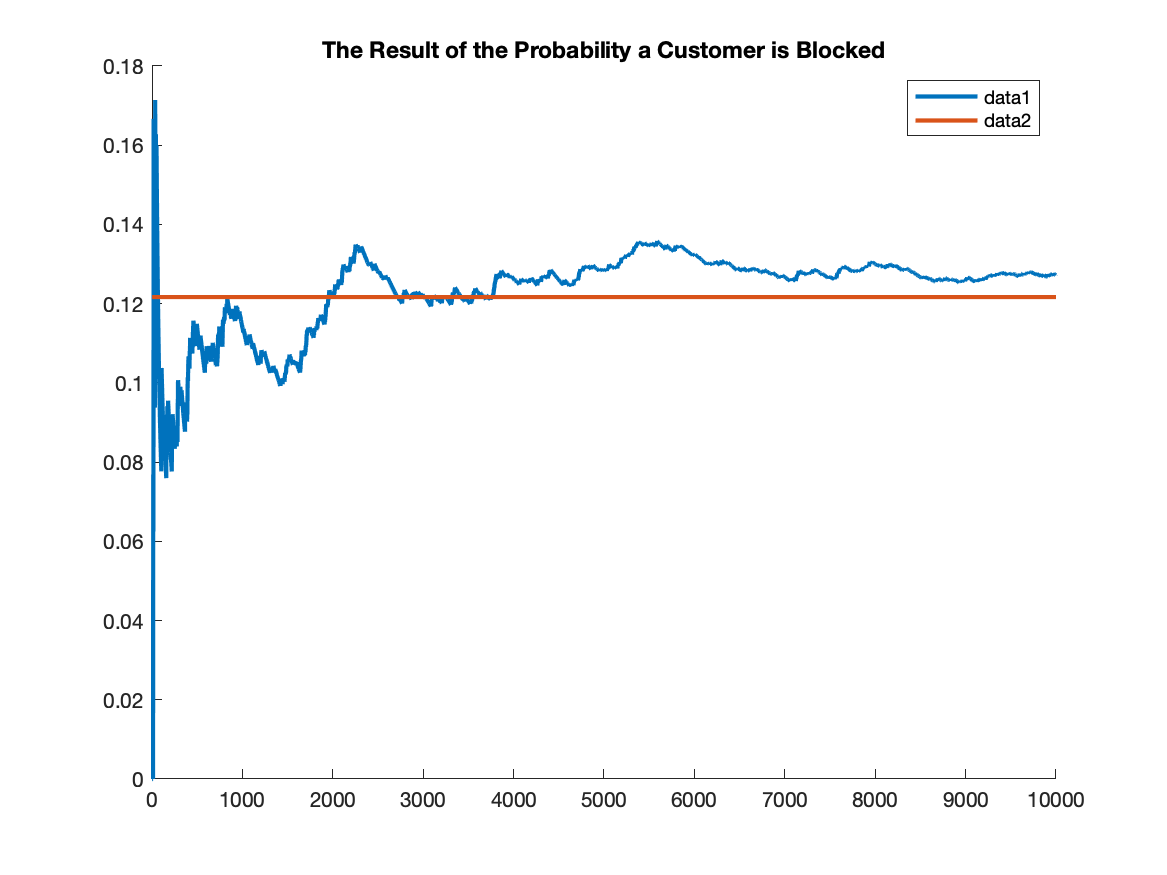
\includegraphics[scale=0.4]{Figures/figure4_2.png}\\
    \figuretitle{Figure 12: The result of the probability a customer is blocked.}
\end{center}\\
\\


%\begin{table}[h!]
%\centering
%\caption{Discrete Event Simulation of Blocking System .}
%\label{summstats}
%\begin{tabular}{|l|c|c|c|c|c|c|c|}
%\hline
%\textbf{Series}  & \multicolumn{1}{l|}{\textbf{Inter-Arrival Time}} & \multicolumn{1}{l|}{\textbf{Service Time}}& %\multicolumn{1}{l|}{\textbf{Mean}}& \multicolumn{1}{l|}{\textbf{Variance}}& \multicolumn{1}{l|}{\textbf{Lower Bound}}& %\multicolumn{1}{l|}{\textbf{Upper Bound}} & \multicolumn{1}{l|}{\textbf{elapsed time}}\\ \hline

   % Analysis      & \exp{1}& \exp{8}   & 0.121661  & - & -         & -        & -       \\ \hline
   % 1 &  exp(1)   & exp(8) & 0.121679  & 0.000040  & 0.121428  & 0.121930 & 23.269 s \\  \hline
   % 2 & Erlang(1) & exp(8) & 1.000343  & 0.000020  & 1.000164  & 1.000523 & 39.241 s \\  \hline
    %3 & he(0.8-0.833, 0.2-5.0) & exp(8) & 4.163967  & 0.002352  & 4.162038  & 4.165897 & 24.459 s \\  \hline
    %4 & exp(1)    & cons(8) & 0.999592  & 0.000081  & 0.999234  & 0.999951 & 16.072 s \\  \hline
    %5 & exp(1)    & Pareto(1.05, 0.38) & 1.001194  & 0.000071  & 1.000859  & 1.001529 & 17.601 s \\  \hline
    %6 & exp(1)    & Pareto(2.05, 4.10) & 0.998682  & 0.000109  & 0.998267  & 0.999098 & 19.684 s \\  \hline
%\end{tabular}
%\end{table}\\
\\

\section{Exercise 5: Variance reductions method}
Variance reduction is a procedure used to increase the precision of the estimates that can be obtained for a given simulation, in order to make a simulation statistically efficient and obtain a greater precision and smaller confidence intervals for the output random variable of interest, variance reduction techniques can be used.The aim of this exercise is using some methods such as Antithetic variables, Control variates, Stratified sampling and importance sampling for variance reduction.
\subsection{The crude Monte Carlo estimator}
We want to estimate $\int_0^1 e^{x}dx$ by using crude Monte Carlo estimator based on 100 samples and present the result as the point estimator and a confidence interval.\\
This integral can be interpreted as
\begin{equation}
    E(e^U)=\int_0^1 e^{x}dx=\theta,        U\in U(0,1)
\end{equation}
TO estimate the integral,we sample of the random variable $e^U$ $(x_{i}=e^U_{i}$ and we take the average,\\
\begin{equation}
    \overline{X}=\frac{\Sigma^{i=1}_{n}X_i}{n}
\end{equation}
\subsection{Antithetic variables}
As mentioned before, doing simulation for estimating parameter $\theta=\overline{X}$ is more efficient if $Var(X)$ is reduced. Let identically distributed random variables $X_1$ and $X_2$ is generated then
\begin{equation}
    Var(\frac{X_1+X_2}{2})=\frac{1}{4}[var(X_1)+var(X_2)+2 Cov(X_1,X_2)]
\end{equation}
Variance is reduced if  $X_1$ and $X_2$ have $Cov(X_1,X_2)\leq 0$.
We want to estimate $\int_0^1 e^{x}dx$ by using Antithetic variables
\subsection{Stratified sampling}
Stratified random sampling is a method of sampling that involves the division of a population into smaller sub-groups known as strata. In  Stratified sampling members, the strata are formed based on shared attributes or characteristics such as income or educational attainment.\\
\\Table 5 shows the estimation of the integral for 3 different methods which is presented in sections 5.1, 5.2 and 5.3.

\subsection{Control variates}

In this part of exercise we used control variates to reduce the variance of the estimator in exercise 4 (Poisson arrivals).\\
Table 6 shows control variates which reduce the variance of the estimator in exercise 4.

\subsection{Simulation Result}

\begin{center}
    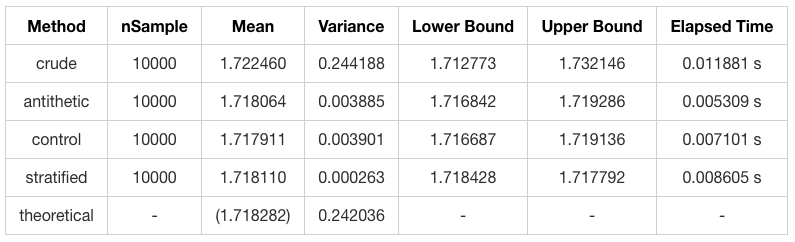
\includegraphics[scale=0.55]{Figures/figure5_1.png}\\
    \figuretitle{Table 5: Estimation of the integral by simulation. Present the point estimator and confidence interval.}
\end{center}\\

\begin{center}
    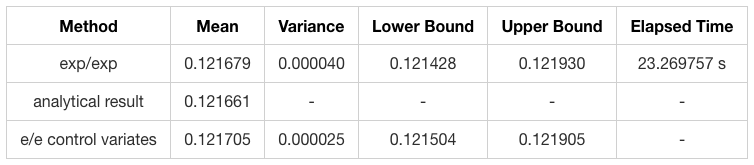
\includegraphics[scale=0.55]{Figures/figure5_2.png}\\
    \figuretitle{Table 6:Control Variates in Exercise 4.}
\end{center}\\
\section{Exercise 6: Markov Chain Monte Carlo}
the aim of this project is simulating the value of a random vector $X$ whose component random variables are dependent. Markov chain Monte Carlo (MCMC) method is a powerful approach for generating a vector whose distribution is approximately of $X$. MCMC comprise a class of algorithms for sampling from a probability distribution. By constructing a Markov chain that has the desired distribution as its equilibrium distribution, one can obtain a sample of the desired distribution by observing the chain after a number of steps. The more steps there are, the more closely the distribution of the sample matches the actual desired distribution.\\
\subsection{Metropolis-Hastings algorithm}
Metropolis–Hastings algorithm is a Markov chain Monte Carlo (MCMC) method for obtaining a sequence of random samples from a probability distribution from which direct sampling is difficult. This sequence can be used to approximate the distribution.

First part of this exercise, we generate Random Walk Metropolis-Hastings (RW-MH) Simulation of the Queue Problem.

\begin{center}
    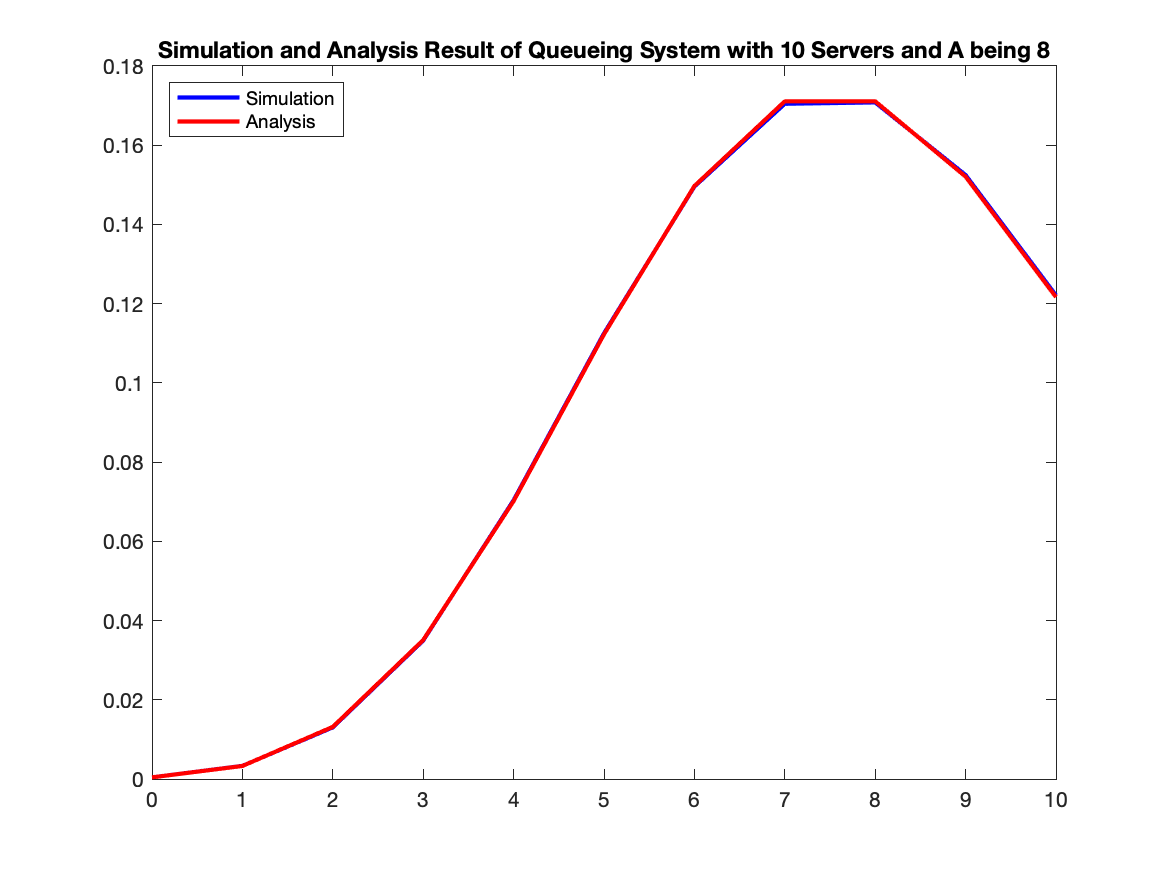
\includegraphics[scale=0.6]{Figures/figure6_1.png}\\
    \figuretitle{Figure 13: Simulation and analysis result of queuing system with 10 servers and A being 8.}
\end{center}

\subsection{Metropolis-hasting with two dimensional}
we want to use Metropolis-Hastings, directly and coordinate wise to generate variates from this distribution. we use $A1,A2 = 4$
and $n = 10$.

Figure 11 shows simulation and analysis result of generating values by Metropolis-Hastings algorithm in one dimensional.

\begin{center}
    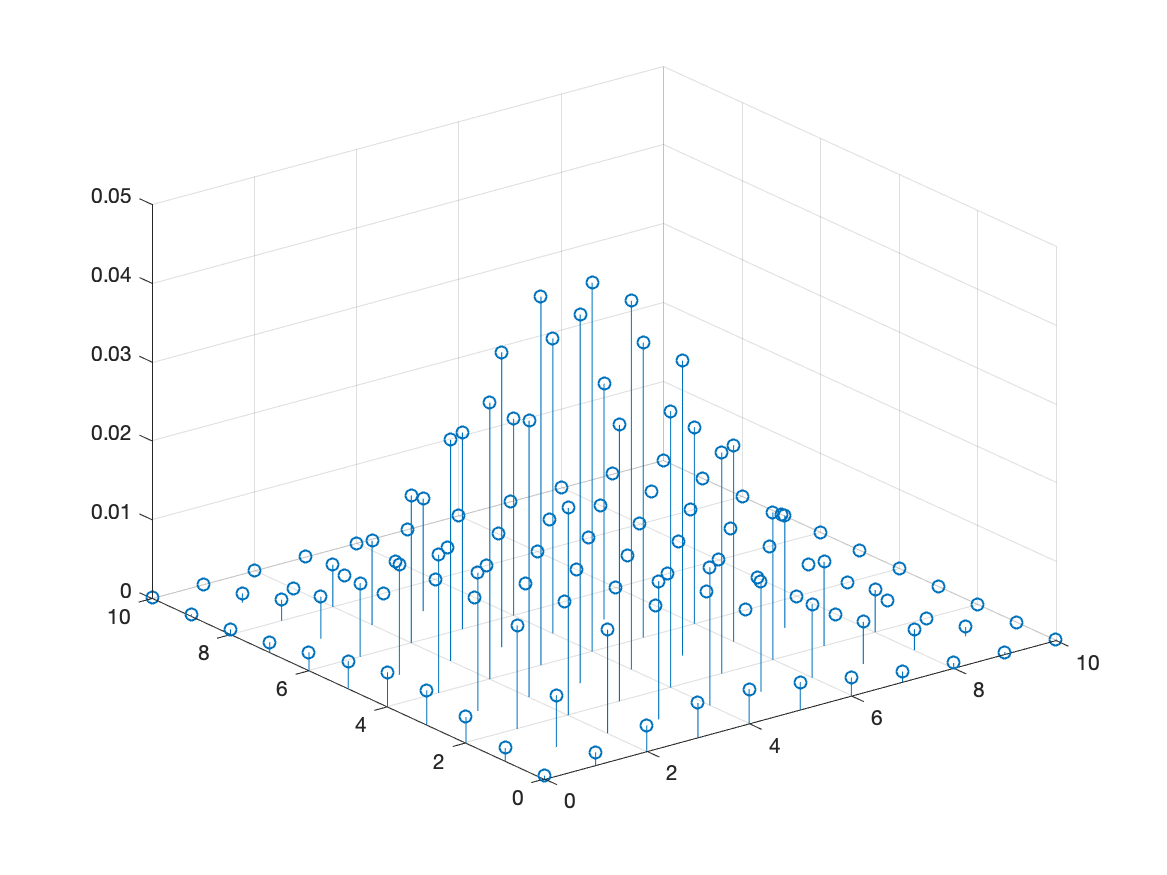
\includegraphics[scale=0.6]{Figures/figure6_2.png}\\
    \figuretitle{Figure 14: Analytical Result of Two-Dimension Problem.}
\end{center}

A algorithm for direct Metropolis-Hastings of two-dimension problem is implemented, which can be called "Array the 2-D Irregular Sample Space for 8-Direction Random Walk". The sample space like the following one is caused by the external conditions. So we have to find all the combinations in the sample space, and sort them randomly:

(0, 3) \\
(0, 2) (1, 2) \\
(0, 1) (1, 1) (2, 1) \\ 
(0, 0) (1, 0) (2, 0) (3, 0) \\

(0, 2) (0, 3) (2, 0) (3, 0) (1, 1) (0, 0) (2, 1) (1, 0) (1, 2) (0, 1)

Then, we array the sample space to rectangle, where we can perform two-dimension random walk. The head and tail of every column, row are connected respectively, so the random walk will not exceed the boundary:

(0, 2) (0, 3) (2, 0) (3, 0) (1, 1) \\ 
(0, 0) (2, 1) (1, 0) (1, 2) (0, 1)

The above illustration is a simple one, while this problem has 66 combinations in total in sample space. The effect of the random walk is shown in the following figure.

\begin{center}
    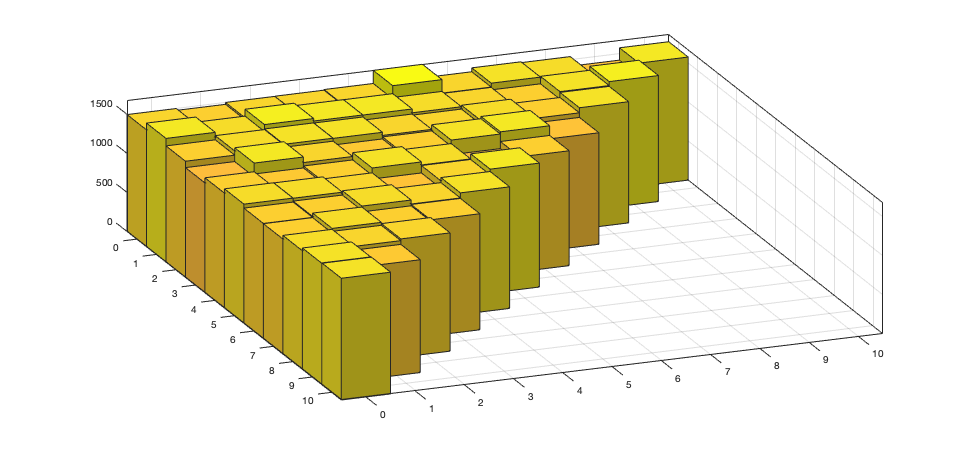
\includegraphics[scale=0.6]{Figures/figure6_7.png}\\
    \figuretitle{Figure 14: Direct Metropolis-Hastings of Two-Dimension Problem.}
\end{center}

Figures 15 and 16 present the generation of values by Metropolis-Hastings, directly and coordinate wise respectively. The red point the theoretical value. It can be seen that the algorithm works very well, and the statistical test result is shown in table 7.

\begin{center}
    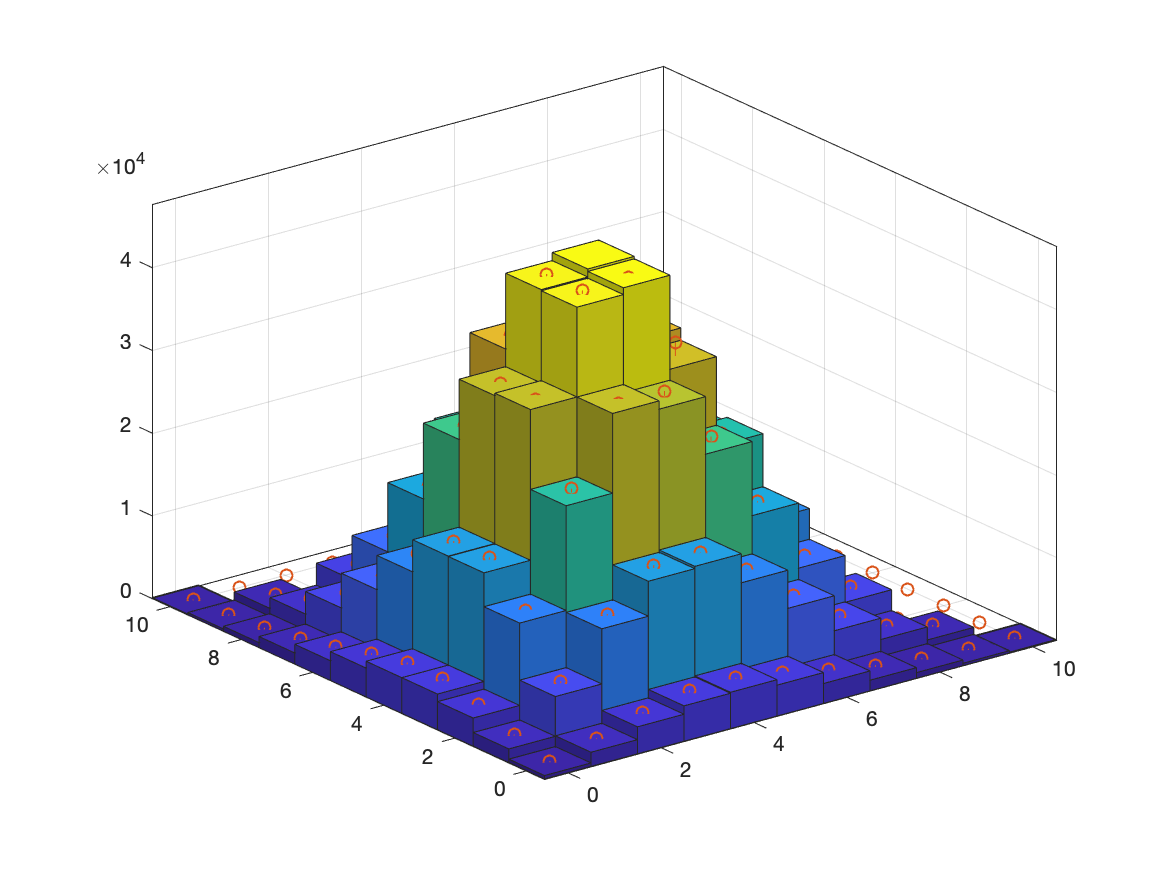
\includegraphics[scale=0.6]{Figures/figure6_3.png}\\
    \figuretitle{Figure 15: Direct Metropolis-Hastings of Two-Dimension Problem.}
\end{center}

\begin{center}
    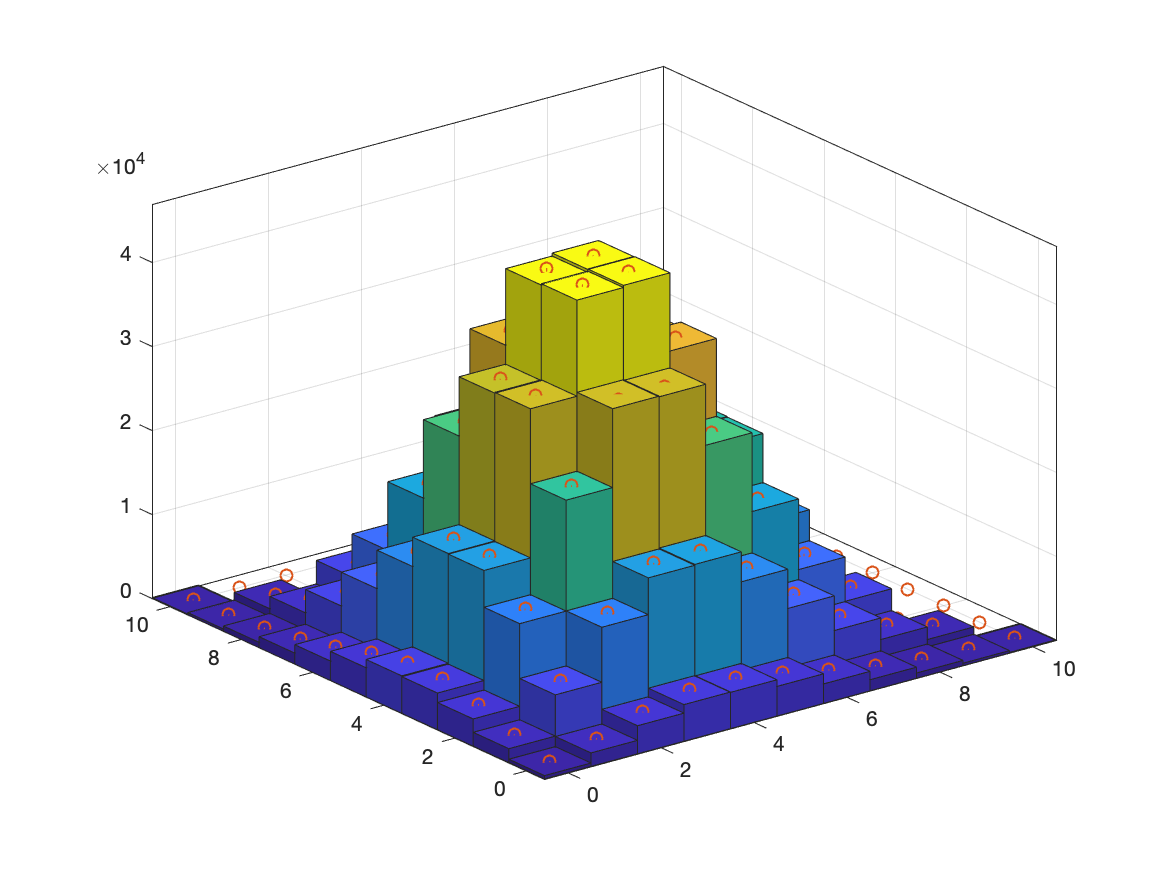
\includegraphics[scale=0.6]{Figures/figure6_4.png}\\
    \figuretitle{Figure 16: Coordinate-Wise Metropolis-Hastings of Two-Dimension Problem.}
\end{center}

\subsection{Gibbs sampling}
Gibbs sampling is a Markov chain Monte Carlo (MCMC) algorithm for obtaining a sequence of observations which are approximated from a specified multivariate probability distribution, when direct sampling is difficult. This sequence can be used to approximate the joint distribution or the marginal distribution of one of the variables.\\
The Gibbs sampling assumes for any $i,i=1,...,n$ and any values $x_j$, $j\neq i$, we can generate random variable $X$ having the probability mass function

\begin{equation}
    P\{X=x\} = P\{X_{i}=x|X_{j}=x_{j},j\neq i\}
\end{equation}

\begin{align}
    P(i, j) &= \frac{1}{K} \frac{A_1^i}{i !} \frac{A_2^j}{j !} = \frac{g(i, j)}{K} \qquad 0 \geq i + j \geq 10 \\
    P\{X=x\} &= P\{X_{i}=x|X_{j}=x_{j},j\neq i\} = \frac{P\{X_{i}=x, X_{j}=x_{j},j\neq i\}}{P\{X_{j}=x_{j},j\neq i\}} \\
    P\{X=x\} &= \frac{g(x, x_{j})}{\sum_{k = 0}^{10 - x_{j}} g(k, x_{j})} = \frac{A_1^x}{x !} L_{x_{j}} \qquad L_{x_{j}} =  \frac{ A_2^{x_{j}}}{ x_{j} ! \sum_{k = 0}^{10 - x_{j}} g(k, x_{j})} 
\end{align}

Figure 17 shows coordinate wise solution using Gibbs sampling.

\begin{center}
    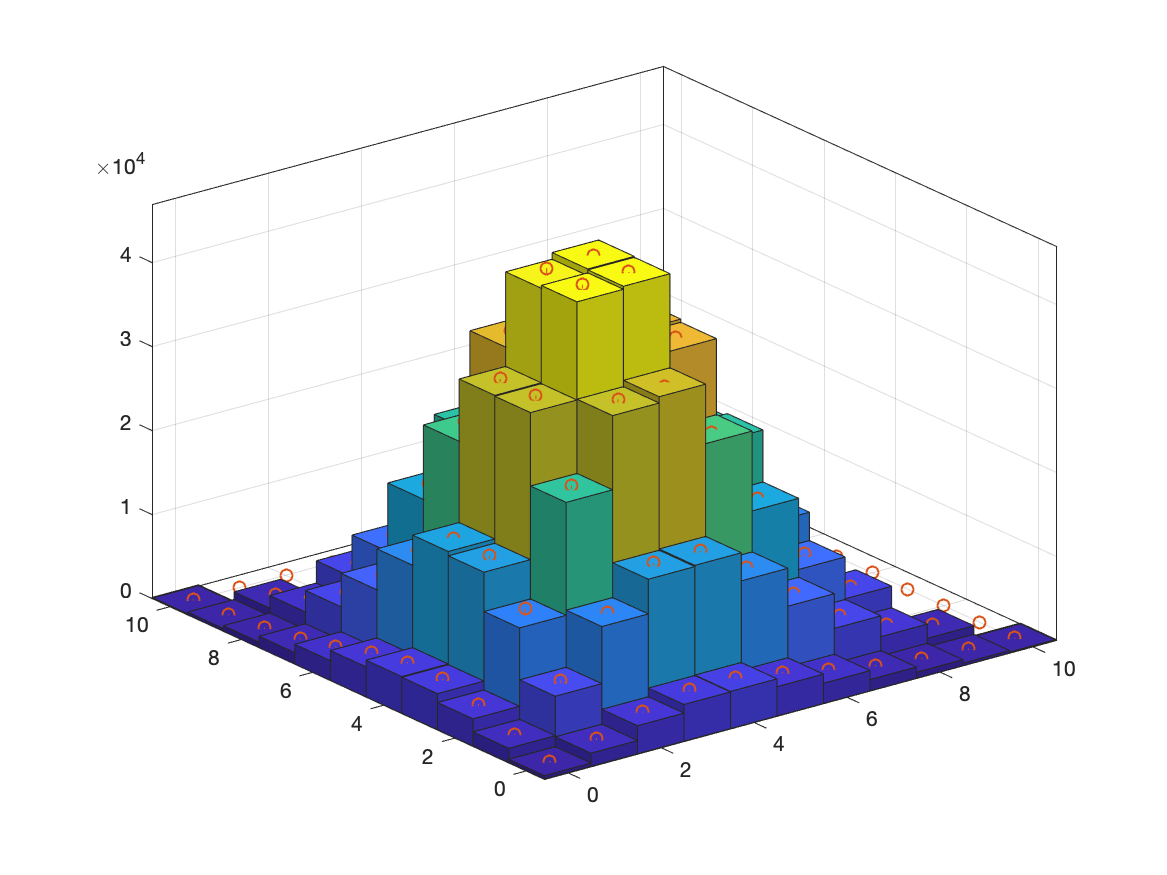
\includegraphics[scale=0.5]{Figures/figure6_5.png}\\
    \figuretitle{Figure 17:Coordinate wise Gibbs sampling .}
\end{center}\\
\\
Table 5 show $\chi^2$ values and Critical $ \chi^2$ values for 4 different methods.\\
\begin{center}
    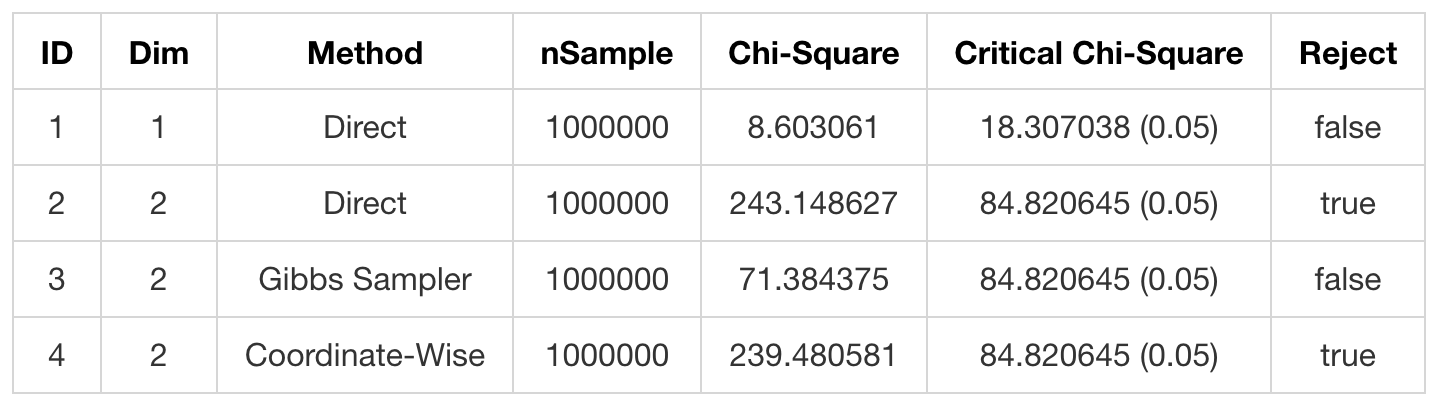
\includegraphics[scale=0.5]{Figures/figure6_6.png}\\
    \figuretitle{Table 7:results of $\chi^2$ Test for different methods .}
\end{center}\\
\section{Exercise 7: Simulated annealing}
Simulated annealing is a probabilistic technique for approximating the global optimum of a given function, in other word,it attempts to find the global optimum in presence of multiple local optima.\\
The aim of this exercise is finding a route S (a permutation of $1, . . . , n$) with minimal total cost $\Sigma^{i=1}_{n_1}A(S_{i},S_{i+1})$ in Travelling salesman problem (TSP) with Given n stations, and an n-by-n matrix A giving the cost of going
from station i to j, which starts and ends at station 1, $S1 = 1$.\\

Three parameters "tempMax", "coefDecay" and "coefStretch" are added in the function to calculate the decreasing temperature. The main purpose is to lower the annealing speed, which allows more "jumping" from the local optimal in the early stage.

\begin{lstlisting}
function [temp] = calTemp(k, tempMax, coefDecay, coefStretch)
    temp = tempMax / (1 + coefStretch * k)^coefDecay;
end
\end{lstlisting}

\begin{center}
    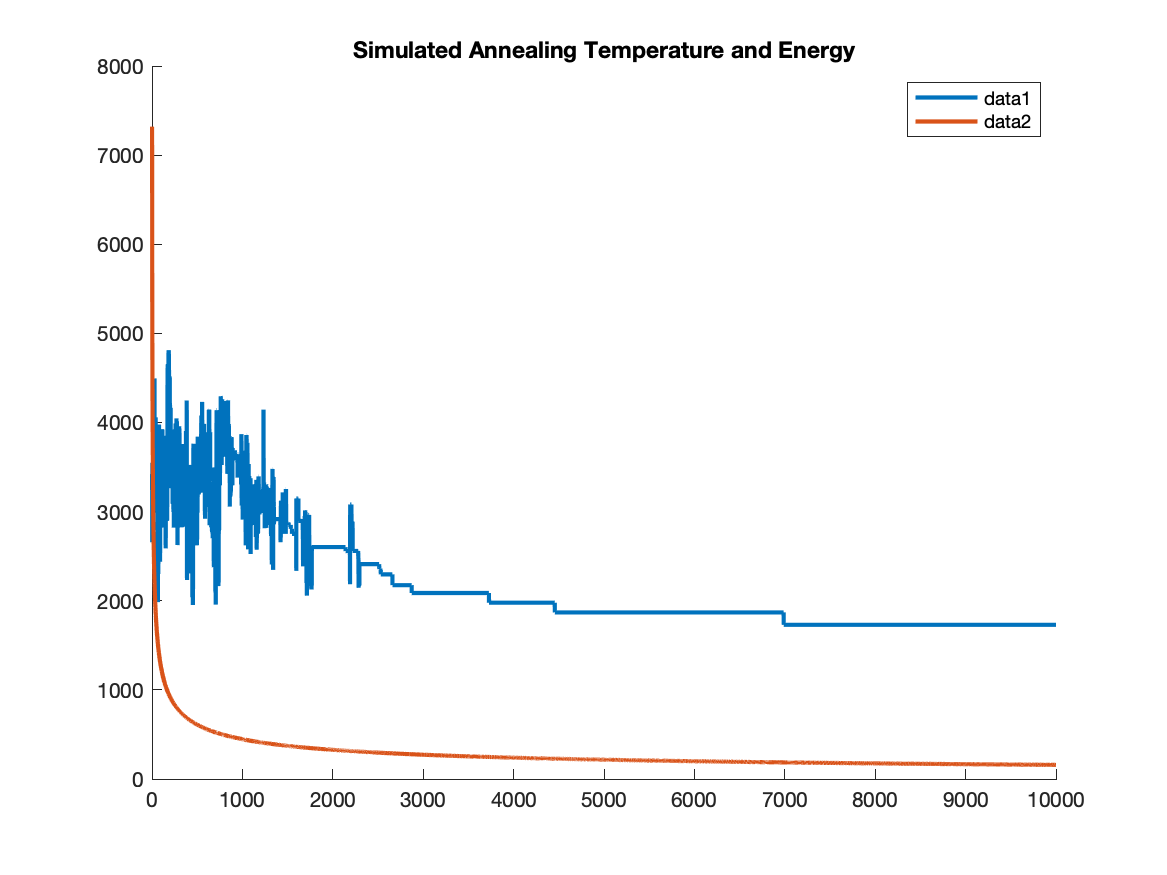
\includegraphics[scale=0.5]{Figures/figure7_3.png}\\
    \figuretitle{Figure 18: simulated Annealing temperature and energy.}
\end{center}\\

Once there are enough "jump" for searching, we extend the simulation times to try to get better result.

\begin{center}
    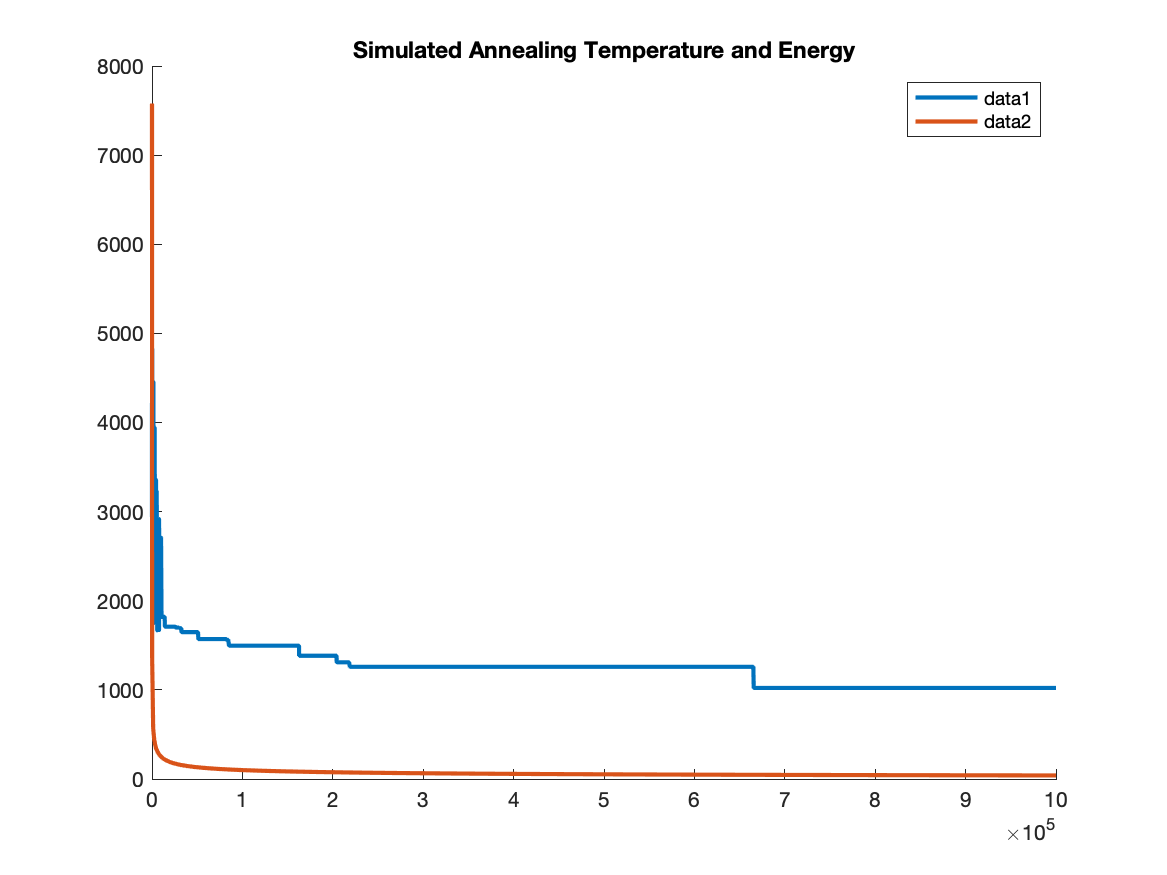
\includegraphics[scale=0.5]{Figures/figure7_1.png}\\
    \figuretitle{Figure 19: simulated Annealing temperature and energy.}
\end{center}\\

The final result from experiment is shown in the following table:

\begin{center}
    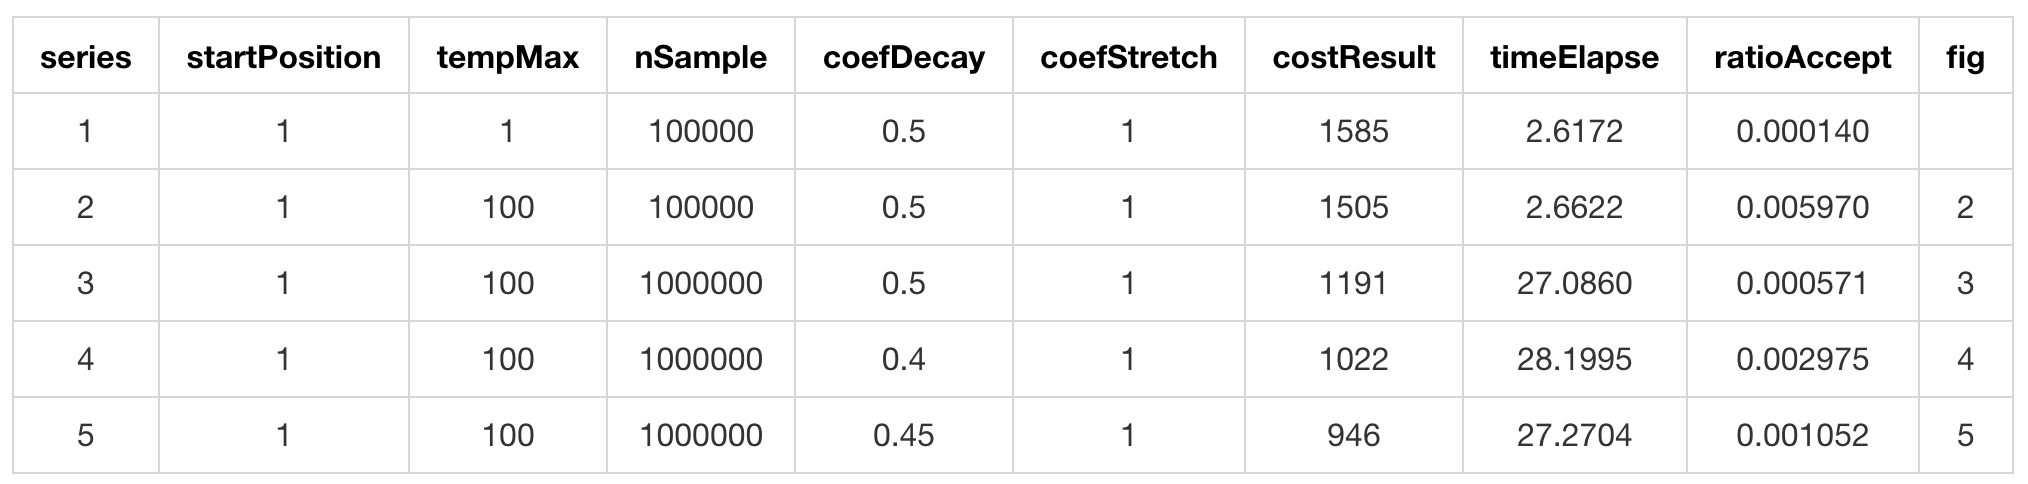
\includegraphics[scale=0.5]{Figures/figure7_2.png}\\
    \figuretitle{Table 8: Optimization Result.}
\end{center}\\
\section{Exercise 8: Bootstrap}
The Bootstrap method is a technique for estimating the variance or median of an estimator based on sampling from the empirical distribution.\\
The aim of this exercise is using Bootstrap method to estimate variance of the estimator(according lecture 10). In this respect, at first we Simulate r  data sets, each with N “observations” sampled form the empirical distribution $F_e$.\\
For each simulated data set, estimate the parameter of interest. This is a bootstrap replicate of the estimate.\\
Finally report the variance among the bootstrap replicates.\\
\\In this exercise we write a subroutine that takes as input a “data” vector of observed values, and which outputs the median as well as the bootstrap estimate of the variance of the median, based on r = 100 bootstrap replicates.\\
\\For testing, we Simulate $n = 200$ Pareto distributed random variates with $\beta = 1$ and $k = 1.05$.\\
Table 7 show the Computation of the mean, the median, and the bootstrap estimate of the variance of the sample median.

\begin{center}
    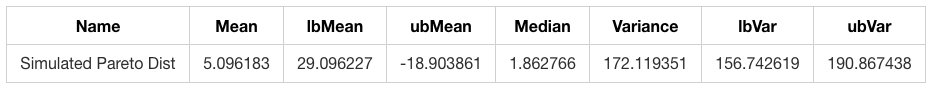
\includegraphics[scale=0.5]{Figures/figure8_2.png}\\
\end{center}\\

\begin{center}
    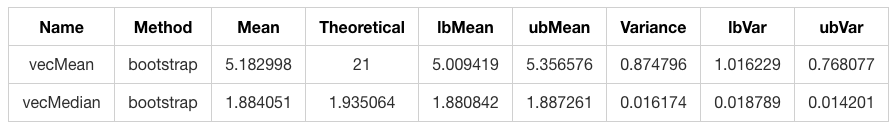
\includegraphics[scale=0.55]{Figures/figure8_1.png}\\
    \figuretitle{Table 9: Bootsrap Result .}
\end{center}\\

From table 9, we can see that the bootstrap method can be used to estimate the sample median. The variance and confidence interval of median can also be calculated, which shows that the estimation is very accurate. For Pareto distribution, it's hard to get the precise mean. Even the variance of the estimated mean from 100 sets is large.
\clearpage
\appendix
\section{Appendix: MATLAB codes}
\subsection{Exercise 1} \label{app:main}
\lstinputlisting{Matlab/Exercise1.m} 
\subsection{Exercise 2} \label{app:main}
\lstinputlisting{Matlab/Exercise2.m} 
\subsection{Exercise 3, 4, 5, 6, 7, 8}
See folder "code" in zip. The setup file is "setup.m". All the result is in "results" folder.
\newpage
%\bibliography{references.bib}
\printbibliography
\end{document}























